\chapter{Routing protocols in Wireless Sensor Network with Holes}\label{chapter3}
We noted that the existence of routing holes in network's topology usually causes the local minimum phenomenon. Thus, a routing protocol has only two options in this scenario, either to drop the packet or to solve the routing hole problem, by using a certain mechanism. There are different methods of dealing with this problem. These protocols have helped us to further define some aspects of our design for the near hole routing protocol. In this chapter, we present these works, and point out their advantages that have been derived in our proposed protocol. 

To approximate the hole polygon, firstly, we have to detect the hole boundary, or, those nodes that lie on the boundary of the hole. This problem is known as the hole boundary detection problem. The detection of hole boundary is important for improving wireless sensor networks operations. 

There is an intuitive way to detect a routing hole. Given a network presented as a Cartesian coordinate system in which each sensor node is a point in the plane, we construct Delaunay triangulation of this network, then with a pre-defined threshold $\eta$, we remove all edges whose length is greater than $\eta$. Remaining edges create some polygons which have more than 3 edges. These polygons may be routing holes. However, the problem of this algorithm is that it is not a distributed protocol, since it requires a central node that has location information of all sensor nodes in the network. Hence, applying this algorithm in case of wireless sensor network may not be effective. Some distributed version of Delaunay triangulation have been proposed, but according to our current knowledge, there is still no truly distributed algorithm.

In 2004, Q.Fang proposed a novel algorithm called \emph{BOUNDHOLE} to detect the hole boundary in a distributed manner. Many routing protocols have adopted the \emph{BOUNDHOLE} algorithm for their hole boundary detection phase. In this chapter, before going into detail of current proposed routing protocols, we will give an overview of \emph{BOUNDHOLE} algorithm.
\section{The TENT rule and BOUNDHOLE algorithm} \label{chapter3.1-boundhole}
\subsection{The TENT rule}
The \emph{TENT rule} is used locally by each sensor node, that is, a node $p$ needs only its 1-hop neighbors and itself location information to determine whether it lies on the boundary of a routing hole. We exemplify the \emph{TENT rule} using representation in figure \ref{tent-rule}. At each node $p$, its neighbors are sorted angularly. For every pair of neighbors $u$ and $v$, where $\overrightarrow{pu}$ is left of $\overrightarrow{pv}$, we consider the perpendicular bisectors of each link (labeled $l1$ and $l2$ in figure \ref{tent-rule}). If the intersection of the bisectors falls outside of the range of $p$, then $p$ has no neighbors closer to the region bounded by the communication range and the bisectors (i.e., the black region in figure \ref{tent-rule}). $p$ is called \emph{``stuck node''} and $\angle upv$ is called \emph{``stuck angle''}. Note that this method locates regions, rather than nodes, where no neighbors are closer. Every node must evaluate its 1-hop neighbors using the \emph{TENT rule}, and only at nodes that the \emph{TENT rule} fails may packets get stuck. If a node $p$ has at least 1 stuck angle, $p$ has to be on the hole boundary. 

This rule also elicits that if angle $upv$ is less than $120\degree$, then there is no stuck angle of $p$ corresponding with pair $(u,v)$. Thus, a sensor node has at most 3 stuck angles.

Upon detecting a failure, stuck nodes are responsible for initiating the \emph{BOUNDHOLE} algorithm.

\begin{figure}[!htb]
\centering
\includegraphics[width=0.4\textwidth]{Chapter3/Chapter3Figs/fig-stuck-node.png} % strongly stuck node
\caption{TENT rule: Node $p$ has no neighbors closer to the back regions as determined by the intersection of bisectors of adjacent links.}
\label{tent-rule}
\end{figure}

\subsection{The BOUNDHOLE algorithm}
After being detected as a \emph{stuck node}, the stuck node $p$ can initiate the distributed algorithm, \emph{BOUNDHOLE} that uses the right-hand rule to connect a node with its neighbors, to form a closed region. That closed region is a routing hole. The basic idea is shown in figure \ref{boundhole}. The algorithm starts from node $p$ and sweeps over the stuck direction by sending a packet to node $t_1$ in a counter-clockwise direction. Node $t_1$ then passes the packet to node $t_2$. The above process is repeated until the packet moves around the hole boundary and returns to $p$. Now that the boundary of a hole has been identified and stored locally. 

\begin{figure}[!htb]
\centering
\includegraphics[width=0.4\textwidth]{Chapter3/Chapter3Figs/fig-boundhole.png} % strongly stuck node
\caption{BOUNDHOLE algorithm: Greedy sweeping at $t_1$}
\label{boundhole}
\end{figure}

A stuck node initiates a messenger packet in each direction this node is stuck in. Thus, there are a lot of packets the originated from all stuck nodes in the hole boundary. These packets are obviously redundant since we need only 1 packet to detect the hole boundary. To reduce networking overhead and possible packet collisions, especially when large holes exist in the network, the ID of the originator is recorded in each messenger packet and the messenger packet originated by the stuck node with the lowest ID is guaranteed to be overlaid at each hop. That is, all packets which have the originator ID greater than the lowest ID will be dropped.

Due to the distributed property of the \emph{TENT rule} and the \emph{BOUNDHOLE} algorithm, this protocol ensures the scalability even when the network topology is extended.

\section{Hole bypassing protocols}
As stated previously, all the proposed routing protocols using the \emph{BOUNDHOLE} algorithm in its hole boundary detection phase construct a forbidden area which covers the hole polygon. The purpose of constructing these forbidden areas is to simplify the hole polygon, thus it reduces the memory and network overhead for storing and broadcasting the hole information to the network. The forbidden area could be represented as a simpler shape such as circle \cite{ehds}, ellipse \cite{ellipse}, hexagon \cite{hexagon}, parallelogram \cite{elbar} or octagon \cite{issnip}. We call these simpler shapes are the approximate hole. These protocols are all separated to 2 main phases. The first one is the network initialization phase, and the second one is data forwarding phase. However, there are some fundamental differences among these protocols. 

In the network initialization phase, all mentioned protocols try to detect the hole boundary using the \emph{BOUNDHOLE} algorithm. After finishing detecting the hole boundary, the hole boundary message originator calculates the approximate holes. After that, some protocols (which are \cite{ellipse}, \cite{hexagon}, \cite{elbar}, \cite{issnip}) have an extra phase called broadcast hole information phase. The broadcast data could be the information of the approximate hole, and the broadcast area is controlled by a system parameter. In the contrary, some protocols (which are \cite{ehds}) forward the hole information to all boundary sensor nodes, and let each boundary sensor node calculate the approximate hole itself.

In the data forwarding phase, although each protocol uses a different shape of forbidden area, the routing path construction algorithm still shares some common ideas. They all use the concept of \emph{virtual anchor point}. These \emph{virtual anchor points} create a hole-bypassing routing path for the data packet, and its determination depends on each routing protocol. There are two common approaches to determine these \emph{virtual anchor points} which are: intersection points of tangent lines in case of \cite{ehds, ellipse} or vertices of approximate polygon in case of \cite{elbar, issnip, hexagon}. 

Due to the limitation of the thesis, we only give thorough studies on \cite{ehds,issnip,elbar} protocols.

%%% EHDS %%%
\subsection{The Efficient Hole Detour Scheme}
A representative for the group using the tangent line to construct the routing path is the Efficient Hole Detour Scheme (\emph{EHDS} protocol). In this proposal, the authors used a circumscribed circle to approximate the hole polygon.

In the network initialization phase, the protocol uses the \emph{BOUNDHOLE} algorithm to detect the hole boundary. Then the creator of the hole boundary detection message calculates the circumscribed circle of the hole polygon using the algorithm described in algorithm \ref{algo-circle}. This circumscribed circle information would be sent to all hole boundary sensor nodes. Figure \ref{fig-circle} represents the idea of this scheme. 

\begin{figure}[!htb]
\centering
\includegraphics[width=0.6\textwidth]{Chapter3/Chapter3Figs/fig-circle.png}
\caption{The Efficient Hole Detour Scheme (cited from \cite{ehds}). Illustration for the hole approximation phase.}
\label{fig-circle}
\end{figure}

\begin{algorithm}[!htb]
\SetAlgoLined
\caption{Circumscribed circle constructing algorithm}
\label{algo-circle}
\Input{ $P=\left \{ P_1, ..., P_n \right \}$: the hole polygon}
\Output{$S(C, r)$: the circumscribed circle of $P$}

$X \leftarrow \{P_{i_x} \mid i = \overline{1,n}\}$\;
$Y \leftarrow \{P_{i_y} \mid i = \overline{1,n}\}$\;
$x_{min} \leftarrow min(X)$ \;
$x_{max} \leftarrow max(X)$ \;
$y_{min} \leftarrow min(Y)$ \;
$y_{max} \leftarrow max(Y)$ \;

$C \leftarrow (\frac{x_{min} + x_{max}}{2}, \frac{y_{min} + y_{max}}{2})$\;
$r \leftarrow \frac{\sqrt{(x_{min} - x_{max})^{2} + (y_{min} - y_{max})^{2}}}{2}$\;
\Return $S(C,r)$\;
\end{algorithm}

In the data forwarding phase, the packets are firstly forwarded by the greedy routing until it reaches a hole boundary sensor node. This node is called an intermediate node. This intermediate node would send the packet back to the source by greedy routing with extra information including the location of center point and the radius of the hole polygon's circumscribed circle. After finishing receiving back the packet, the source node resends the packet with new bypass routing path to avoid the circle. Figure \ref{fig-circle2} illustrates this routing protocol.

\begin{figure}[!htb]
\centering
\includegraphics[width=0.4\textwidth]{Chapter3/Chapter3Figs/fig-circle2.png}
\caption{The Efficient Hole Detour Scheme (cited from \cite{ehds}). Illustration for the data forwarding phase. The forbidden area is the circumscribed circle of the hole polygon.}
\label{fig-circle2}
\end{figure} 

In this figure, \emph{S}, \emph{D} are the source node and the destination node, respectively. Firstly, \emph{S} greedily forwards the packet until it reaches a node \emph{U} which is a hole boundary sensor. \emph{U} then sends back to \emph{S} the forbidden area information. Finally, \emph{S} re-forwards the packet using new routing path, that is $\overrightarrow{SVD}$. The packet is forwarded along this path. \emph{V} is called the virtual anchor point in this case.

It is obvious that in the \emph{EHDS} protocol, the packet has to be forward twice: in the first time, it is forwarded by the greedy routing, in the second time, it is forwarded by the hole bypassing routing. Consequently, this increases the packet transmission time, as well as the energy consumption of nodes participating in the routing. 

One more problem of \emph{EHDS} protocol is that, this protocol leads to the routing path enlargement problem in case of near hole routing which is demonstrated in figure \ref{fig-circle-problem}.
\begin{figure}[!htb]
\centering
\includegraphics[width=0.4\textwidth]{Chapter3/Chapter3Figs/fig-circle-problem.png}
\caption{The routing path is enlarged in case of near hole routing.}
\label{fig-circle-problem}
\end{figure}

In this figure, the source node \emph{S} is close to the forbidden area. Since this protocol uses the tangent line as the routing path, the closer to the forbidden area the source node and the destination node are, the more longer the routing path is.

More importantly, the author ignored the case where the source node or the destination node or both of them are inside the forbidden area. In such a case, there is no hole bypassing routing paths.

%%% ELBAR %%%
\subsection{The Energy Efficient and Load Balanced Distributed Routing Scheme}
The Energy Efficient and Load Balanced Distributed Routing Scheme (ELBAR protocol) is the one that simultaneously considers both energy efficiency and load balancing requirements. 
In this protocol, the authors proposed a novel algorithm to approximate the hole polygon. Instead of using a geometric shape, the authors use a square grid to approximate the hole \cite{gridoffline}. Using a square grid ensures the convex/concave properties of the original hole polygon, and the error between the approximate hole and original hole is controlled by a system parameter which is the length of edges of grid's square units. The approximate hole is a polygon whose edges are the edges of the grid and vertices are the vertices of the grid. Its properties are:
\begin{itemize}
\item Covering: the approximate hole covers completely the hole polygon.
\item Controllable approximate error: the upper bound of the total vertices of the approximate hole is controlled by a system parameter $n$. The larger the value of $n$ is, the less the approximate error is.
\end{itemize}

\begin{figure}[!htb]
\centering
\includegraphics[width=0.5\textwidth]{Chapter3/Chapter3Figs/fig-elbar-grid.eps}
\caption{An example of approximate polygon.}
\label{fig-elbar-grid}
\small{Grey area represents the hole. Bold black line represents the boundary of the approximate polygon.}
\end{figure}
Figure \ref{fig-elbar-grid} illustrates the approximate hole using a square grid.

This scheme propose additional modifications to the packet forwarding function and routing functions. With respect to specific routing hole H all the nodes are divided into three regions based on two predefined threshold values $\alpha_{min}$ and $\alpha_{max}$ as shown in figure \ref{fig-elbar-regions}. A particular node is in:
\begin{itemize}
\item region 1 if the hole view angle of the node is either greater than or equal to $\alpha_{max}$,
\item region 2 (which is referred to as an escape region in what follows) if the hole view angle of the node is in interval $(\alpha_{min}, \alpha_{max})$,
\item region 3 if the hole view angle of the node is either less than or equal to $\alpha_{min}$.
\end{itemize}

\begin{figure}[!htb]
\centering
\includegraphics[width=0.5\textwidth]{Chapter3/Chapter3Figs/fig-elbar-regions.eps}
\caption{Regions with respect to a specific routing hole.}
\label{fig-elbar-regions}
\end{figure}

A parallelogram is used as the forbidden area, and these parallelograms are different from each sensor node. The construction of the parallelogram is illustrated in figure \ref{fig-elbar-parallelogram}.

\begin{figure}[!htb]
\centering
\includegraphics[width=0.5\textwidth]{Chapter3/Chapter3Figs/fig-elbar-parallelogram.eps}
\caption{The parallelogram of the sensor node $P$}
\label{fig-elbar-parallelogram}
\end{figure}

The routing protocol is described as follows. Two fields are proposed to be carried by a packet: the first field is the \emph{forwarding mode} that can take either \emph{default} or \emph{escape} value, while the second field \emph{anchor location} is to store the anchor point in the \emph{escape} mode. Let $D$ be the destination of packet $p$. The forwarding mode $p_m$ is initialized to \emph{default} and anchor location $p_a$ takes $D$ when packets are first generated. When node $P$ is in region 3, it simply keeps the \emph{default} mode. When $P$ is in the \emph{escape} region and
\begin{itemize}
\item if $D$ lies either outside the hole view angle of $P$ or inside the hole covering parallelogram at $P$, then the packet is forwarded by the rule of the GPSR protocol \cite{gpsr}.
\item otherwise, a hole escape probability function is executed to adjust the routing mode for the packet. In the escape mode, the route is ``bended'' around $P$’s hole view parallelogram.
\end{itemize}

\begin{figure}[!htb]
\centering
\includegraphics[width=0.5\textwidth]{Chapter3/Chapter3Figs/fig-elbar-routing.eps}
\caption{ELBAR packet forwarding example.}
\label{fig-elbar-routing}
\end{figure}

Figure \ref{fig-elbar-routing} illustrates how a data packet would be routed from source node $S$ in region 3 to destination node $D$. When in region 3 (far from the hole then has no information about it) the packet is forwarded in the \emph{default} mode until it reaches a node in region 2, namely node $S_2$ in the figure. Note that reaching region 2 does not mean automatically switching to \emph{escape} mode but to mean having a chance to switch to this mode. In this example, the adjust routing mode method at $S_2$ returns in \emph{default} mode, thus the packet is forwarded to the neighbor of $S_2$ which is nearest to destination $D$. However, at the next hop, i.e $S_3$, the adjust routing mode method returns in \emph{escape} mode thus $S_3$ updates necessary fields and sends the data packet towards the virtual anchor $A$. Before arriving to the node which is nearest to $A$, the packet however reaches intermediate node $S_n$ that can “see” $D$ (without the view blocking of the hole). Now $S_n$ forwards the packet in the default mode to destination $D$.

In the \emph{ELBAR} protocol, we can think region 1 as the near hole region. For the source node belonging to this region, the \emph{GPSR} routing protocol is used.

%%% ISSNIP %%%
\subsection{The Load Balanced Routing with Constant Stretch Scheme}
The Load Balanced Routing with Constant Stretch Scheme (the \emph{OCTAGON} protocol) takes a further step to target and solve two problems of hole diffusion and path enlargement. Its theoretical analysis proves the constant stretch property and its evaluation results show that this scheme strongly outperforms the existing schemes in several performance factors, including route stretch, efficient use of energy and load balancing.

This protocol also consists of 2 main phases: the initial network setup phase and the data forwarding phase. The initial network setup is designed to produce the core polygon, a compact approximation of the hole, which has 8 vertices and covers the hole boundary. The initial network setup process consists of three sub-phases. First, the nodes on the hole boundary are identified using the \emph{BOUNDHOLE} algorithm \cite{boundhole}. Then, the core polygon is constructed. In the final phase, the core polygon information is disseminated to the nodes surrounding the hole. The dissemination area is not all of the network but only a restricted area in order to save the energy consumption. Once the initial network setup is finished, the nodes nearby the hole know about the location of the core polygon while the nodes far from the hole do not.

If the packet is initialized at a source node out of a dissemination area of a hole(not knowing about the hole and the core polygon), it is simply greedily forwarded towards the destination node until reaching an intermediate node inside this area. Once in this area the source node (or intermediate node) can construct a packet-specific polygon, seen as a forbidding area for this packet, which is the image of the core polygon through a homothetic transformation with the scale factor based on the source-destination distance. The packet is then greedily forwarded to the virtual anchor points which are the vertices of this packet-specific polygon. 

The core polygon satisfies the following conditions:
\begin{itemize}
\item It completely covers (the boundary of) the hole.
\item It has at most 8 vertices and each edge of its contains at least one vertex of the hole.
\item All angles at the vertices that are not the vertices of the hole, equal to $\frac{3\pi}{4}$.
\end{itemize}

After the core polygon information broadcast phase, the network is divided into 2 regions: region 1 contains nodes that receive the hole core polygon broadcast message, and region 2 contains the other nodes as shown in figure \ref{fig-issnip-routing}.

The main idea of the data forwarding phase is to find the shortest route that has to go around a larger polygon $A$ that is the image of the core polygon through a homothetic transformation using a center $I$ chosen randomly inside the core polygon and the scale factor $\xi > 1$ computed based on the distance between the source and the destination. This polygon $A$ is being used as a dynamic forbidding area which is different per each packet and source node because of the randomization of center $I$. As a result, the routing path also changes dynamically for each packet and thus balance the energy consumption of the network. While, the scale factor $\xi$ is designed so that the stretch of the routing path is bounded by a constant. Figure \ref{fig-issnip-routing} shows examples of the routing scheme in both cases when the source node belongs to the region 1 and to the region 2.

\begin{figure}[!htb]
\centering
\begin{subfigure}{0.5\textwidth}
  \centering
  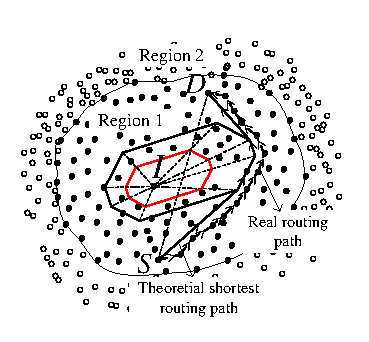
\includegraphics[width=0.8\textwidth]{Chapter3/Chapter3Figs/fig-issnip-routing1.eps}
  \caption{Source node belongs to region 1}
  \label{fig-issnip-routing1}
\end{subfigure}%
\begin{subfigure}{0.5\textwidth}
  \centering
  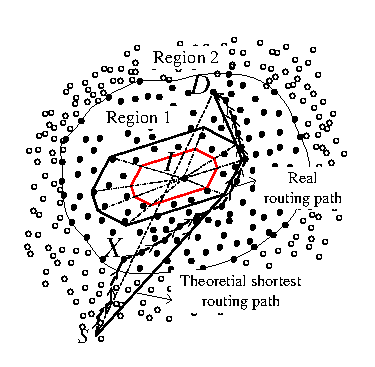
\includegraphics[width=0.8\textwidth]{Chapter3/Chapter3Figs/fig-issnip-routing2.eps}
  \caption{Source node belongs to region 2}
  \label{fig-issnip-routing2}
\end{subfigure}
\caption{Examples of the \emph{OCTAGON} routing scheme}
\label{fig-issnip-routing}
\end{figure}

Since our near hole routing protocol adopted some advantages from this protocol, we give here more details about this protocol's theoretical analysis. Firstly, the authors proved that the upper bound of the stretch does not exceed $\frac{1}{sin(3\pi /8)} + \delta$ for every source and destination pair $(S, D)$ staying outside the core polygon. More notably, the authors explained the reason why they choose a octagon to approximate the forbidden area. The reason is if $P$ is a \emph{n-gon} with equal angles such that $P$ covers the hole and each edge of $P$ contains at least one vertex of the hole, then the E-stretch of $P$ to the hole is bounded by $\frac{1}{sin(\frac{(n-2)\pi}{n})}$, a decrease function which converges to 1. The value of this function decreases strongly when $n$ increases from 3 to 8 and does not decrease much after that.